\chapter{\textbf{Simulation Results}}
\label{chapter:simulation}
In this chapter, we conduct extensive simulations to demonstrate the performance of our proposed online learning algorithm \myalgorithm\ for user-managed SFC placement on edge, in terms of the convergence performance, scalability, and relative performance against other algorithms under varying parameters. All algorithms are implemented in Python 2.7 and run on an Intel Core i5-7400CPU@3.00GHz machine with 8.00 GB RAM. We utilize the Python interface of Networkx \cite{networkx} to simulate customized network and Gurobi \cite{gurobi} to solve the optimal offline optimizations.


% In this chapter, we evaluate our proposed algorithm. We first conduct a set of simulation experiments to show the performance of \myalgorithm under different environmental settings and scalability. Then we validate the algorithm in a \textit{Mininet-wifi} emulation by showing its performance under real environmental dynamics.
\section{Simulation Settings}
\begin{table}
	\centering
	\caption{Simulation parameters}
		\vspace{\baselineskip}
	\label{tab:Simulation parameters}
	% \resizebox{\columnwidth}{!}
	\begin{tabular}{ll}
		\toprule
		Parameter & Value \\[5pt]
		\midrule
		Number of nodes & 26 (25 edge, 1 cloud)\\[5pt]
		
		Edge VNF proc. delay (ms/kbit) & 0.5 - 1 (uniform)\\[5pt]
		Cloud VNF proc. delay (ms/kbit) & 0.1\\[5pt]
		Number of links & 65\\[5pt]
		Link delay (ms) on edge & 10 - 50 (uniform) \\[5pt]
		Link delay (ms) edge2cloud & 100 - 200 (uniform) \\[5pt]
		Migration delay (ms)& 10 - 200 (uniform)\\[5pt]
		VNFs per SFC requests &  3 - 5\\[5pt]
		VNF request (bits) & [250, 2500, 10000]\\[5pt]
		Mobility model & Random Waypoint \\ [5pt]
		
		\bottomrule
	\end{tabular}
\end{table}

\subsection{Network Settings}
We conduct experiments on a simulated 2km $\times$ 2km grid network area with 25 edge nodes and a cloud node, as shown in figure \ref{fig:simtopology}, this setting is in line with \cite{MABserviceplacement}. 
%
Cloud and each edge server is equipped with computation ability, 
The ratio of processing delay factors $\pi_s$ to node capacities is set appropriately to achieve a processing delay of [0.5, 1]  and  0.1 milliseconds per Kbits of data flow for each edge computing node and 0.1 milliseconds per Kbits of data flow for the cloud. 
%
The link delay of user-to-edge and edge-to-cloud links are uniformly distributed in [10, 50] milliseconds and [100, 200] milliseconds, respectively.  The migration delay is proportional to the link delays and thereby is distributed in [10, 200] milliseconds depending on the link that the VNF is migrated through.

%for each edge server, the processing delay is uniformly distributed in [0.5, 1] ms/kbit, and the processing delay on the cloud is 0.1 ms/kbit. The link delay on the edge is uniformly distributed in [10, 50] ms  and the link delay from each edge to cloud is uniformly distributed in [100, 200] ms. we assume that migration delay is proportional to link delay, therefore uniformly distributed in [10, 200] ms depends on the link that the VNF is migrated through. 
We set these values based on~\cite{SFCsettingsapp} so that the environment can provide the conventional end-to-end delays for existing applications (\eg\ web service $500$ms, video streaming $100$ms, and online gaming $60$ms). 

\begin{figure}
	\centering
	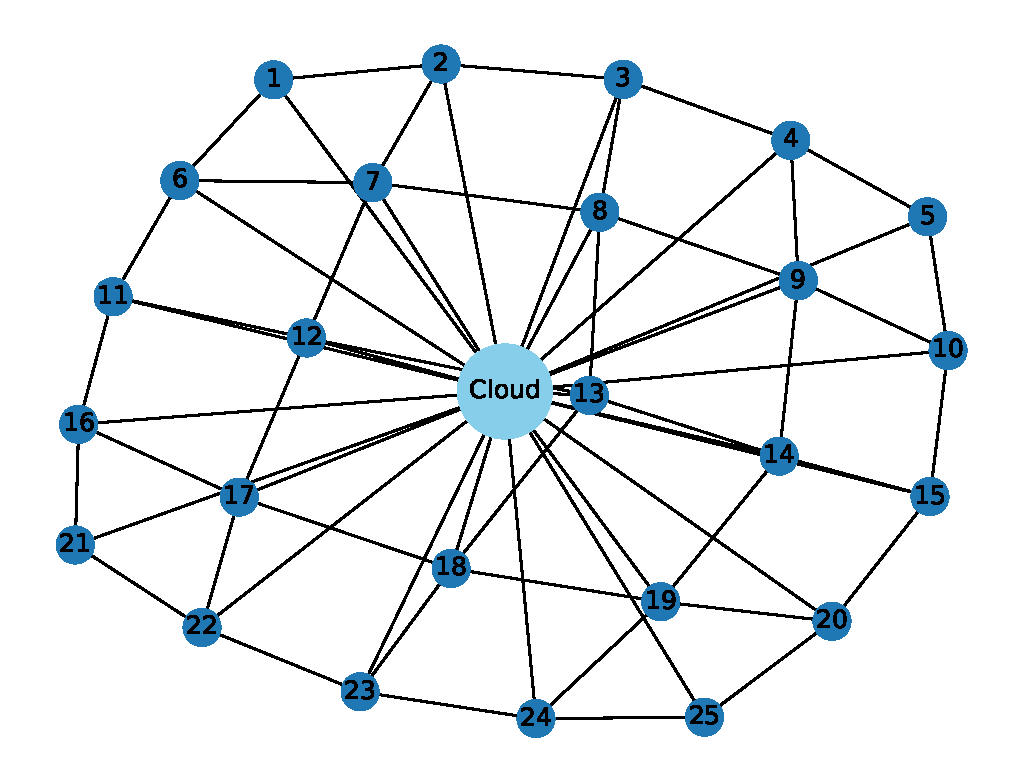
\includegraphics[width=0.9\textwidth]{figs/topology.eps}
		\vspace{\baselineskip}
	\caption{Network topology used in simulation}
	\label{fig:simtopology}
\end{figure}


% For  \textit{networkx}\cite{networkx}. On each node and each link, we add three attributes: actual weight, estimated weight and selected times.
%Actual weights on the nodes are uniformly distributed in  [10, 15] Gbps representing the computing capacity on each nodes, denoted by $c_i$, the capacity on the cloud are set to 100 Gbps. Actual weights on the link represents the
% transmission delay, denoted by $l_{i,j}$. The transmission delay between connected base station or AP is uniformly distributed in [50, 100] ms, the transmission delay to cloud node from each edge node are uniformly distributed in [100, 300] ms. Estimated weights are uniformly distributed in a range based on the actual weight with a noise $n$, that is, $\hat{c}_i^t \sim U(c_i-n, c_i+n)$ and $\hat{l}_{i,j}^t \sim U(l_{i,j} -n, l_{i,j} +n)$, in each timeslot that an arm is being estimated. 



\subsection{SFC Settings}
According to \cite{SFCrequestsetting}, we consider SFC with 3 to 5 different service VNF request. For each request in the SFC, we roughly pick a random choice among three categories: heavy (10000 bytes), medium (2500 bytes), and light (250 bytes) at each timeslot, with regards to the requirements of common service chains such as web services and video streaming, which is summarized in table \ref{tab:SFCexamplereq}.
\begin{table}[htbp]
	\caption{Requirements for common SFCs}
		\vspace{\baselineskip}
	\centering
	\setcellgapes{5pt}\makegapedcells
	\resizebox{\columnwidth}{!}{\begin{tabular}{|c|c|c|c|}
			\hline
			Service Chain & Chained VNFs & Requested Bandwidth &  Maximum Tolerated Latency\\
			\hline
			Web Service  & NAT-FW-TM-WOC-IDPS & 100 kbit/s & 500ms\\
			\hline
			VoIP & NAT-FW-TM-FW-NAT & 64 kbit/s & 100ms \\
			\hline
			Video Streaming & NAT-FW-TM-VOC-IDPS & 4 Mbit/s & 100ms \\
			\hline
			Online Gaming & NAT-FW-VOC-WOC-IDPS & 50 kbit/s & 60ms \\
			\hline
	\end{tabular}}
		\vspace{\baselineskip}
	{\raggedright  \newline
		NAT: \textit{Network Address Translator}, FW: \textit{Firewall}, TM: \textit{Traffic Monitor}, WOC: \textit{WAN Optimization Controller}, IDPS: \textit{Intrusion Detection Prevention System}, VOC: \textit{Video Optimization Controller}  \par}
	\label{tab:SFCexamplereq}
\end{table}

\subsection{User mobility Settings}
To simulate the user's mobility, we use \textit{Random\ Waypoint} mobility model because of its simplicity and wide availability. The random waypoint model has been commonly used as a mobility model in wireless network simulations \cite{bettstetter2004stochastic}. In this model, the user will pause for a fixed number of seconds and then choose a random destination within the network area and a random speed between 1 m/s and 1.5 m/s. The user moves to this destination and again pauses for a period before another random location and speed, as depicted in figure \ref{fig:rwpmodel}. Throughout the movement,
the user is automatically connected to the closest radio base station for communication. 
\begin{figure}
	\centering
	\includegraphics[width=.9\textwidth]{figs/mobilitymodel.PNG}
	\vspace{\baselineskip}
	\caption{Random Waypoint mobility model}
		
	\label{fig:rwpmodel}
\end{figure}


\subsection{Performance Benchmark.}
To evaluate the performance of our algorithm, we compare it to the overall offline optimum that's obtained by solving the optimization formulated in section \ref{section: formulation} using \textit{gurobi}\cite{gurobi}, and the following two edge/cloud-only derivatives of \myalgorithm:
\begin{itemize}
	\item \textbf{Serving on the cloud(SC):} the mobile user would always put the services on the remote cloud to run in order to maximize the computation delay
	\item \textbf{Serving on the edge(SE):} the mobile user would always put the services on the edge servers to run in order to avoid high transmission latency to the cloud. 
\end{itemize}
To show the strength of \myalgorithm\ in terms of scalability, we compare it with the following two greedy learning algorithms:
\begin{itemize}
	\item \textbf{$\epsilon$-greedy.} with a probability of $\epsilon$, randomly choose a super arm, otherwise choose the arm with a maximum average reward
	\item \textbf{Adaptive greedy.} Extension of $\epsilon$-greedy, in which $\epsilon$ is decreasing by time to avoid over-exploring.
\end{itemize}
The parameter used in the simulation is summarized in Table \ref{tab:Simulation parameters}. Nevertheless,  all numeric results are normalized with an appropriate maximum or minimum value from each experiment.


% \begin{figure}
%     \centering
%     \includegraphics[width=0.9\linewidth]{gridsim3.png}
%     \caption{Network topology in simulation}
%     \label{fig:topology simulation}
% \end{figure}
% \subsection{Oracle searching range}
% To explore the optimal oracle search range so that a minimum running time cost is required while the searching area is still wide enough to find the minimal cost, we compare the time cost with service cost within an Oracle at a certain timeslot that has searching range from 1 hop (minimum) to 10 hops (maximum). As shown in figure 7. The optimal service cost can be obtained within minimum two hops while the time cost increases with search range. Therefore setting search range to 2 hops is a optimal solution in our simulation.  

% \begin{figure}
%     \centering
%     \includegraphics[width=0.7\textwidth]{explore.eps}
%     \caption{Exploring Oracle searching range}
%     \label{}
% \end{figure}



% \subsection{\myalgorithm vs. performance benchmark}

% As shown in figure \ref{fig:learningslotbar}, it is easy to find that \myalgorithm algorithm achieves the best performance among other two online algorithms. SE has the worst performance due to the high computation delay on edge.



% \begin{figure}
%     \centering
%     \includegraphics[width=0.9\linewidth]{figs/learningslot1.eps}
%     \caption{The service costs within a certain period}
%     \label{fig:learningslotbar}
% \end{figure}

% \subsection{number of requests}
%\section{Simulation Results}
%In this subsection, we present our simulation results.



\subsection{Impact of network delays}
We considered five levels of computation and transmission delays to investigate their effect on the service quality. 
%We first analyze how the delays (computation delay and transmission delay) in the network setting affect the service performance, and design five levels of computation delay and transmission delay and apply it to the network simulation setting. 
Figure \ref{fig:computingweightbar} and figure \ref{fig:Transmissionweightbar} show that \myalgorithm\ achieves about $15-20\%$ reduction in end-to-end delay compared with other methods. 
For low delays, SE achieves a comparable result because SFCs can be served on the edge with no switching delay due to migration from and to the cloud. SC becomes more competitive when the delays are higher because the computation power of the cloud becomes more significant. Nevertheless, \myalgorithm\ achieves a proper balance between the resources located at the edge and the cloud.



%it is easy to find that \myalgorithm has a overall better performance than the other two derivatives. Specifically, SE has a better performance when either computation and transmission delay is small due to the facts that SFC requests can be served faster on the edge and no switching to the cloud would be involved. However, with the transmission delay or computation delay increasing, it would cost more time to process a SFC request on the edge and thus it has a much worse performance while few performance changes are seen in \myalgorithm and SC.



% \begin{figure}
%     \centering
%     \includegraphics[width=0.9\linewidth]{figs/computationLevel.eps}
%     \caption{Multiple algorithms under different computation settings on edge}
%     \label{fig:computingweightbar}
% \end{figure}

% \begin{figure}
%     \centering
%     \includegraphics[width=0.9\linewidth]{figs/transmissionLevel1.eps}
%     \caption{Multiple algorithms under different transmission settings on edge}
%     \label{fig:Transmissionweightbar}
% \end{figure}

\begin{figure*}[t]
	\centering
	% \begin{subfigure}[b]{.24\textwidth}
	%     \centering
	%     \includegraphics[width=\linewidth]{figs/learningslot2.eps}
	%     \caption{Multiple algorithms under different slots of learning period }
	%     \label{fig:learningslotbar}
	% \end{subfigure}
	\begin{subfigure}[b]{.45\textwidth}
		\centering
		\includegraphics[width=\linewidth]{../icfec21/figs/computationLevel2.eps}
		\caption{Multiple algorithms under different computation settings on edge}
		\label{fig:computingweightbar}
	\end{subfigure}
	\begin{subfigure}[b]{.45\textwidth}
		\centering
		\includegraphics[width=\linewidth]{../icfec21/figs/transmissionLevel2.eps}
		\caption{Multiple algorithms under different transmission settings on edge}
		\label{fig:Transmissionweightbar}
	\end{subfigure}
	% \begin{subfigure}[b]{.45\textwidth}
	%     \centering
	%     \includegraphics[width=\linewidth]{figs/switchingcost2.eps}
	%     \caption{Multiple algorithms under different weights of switching cost}
	%     \label{fig:switchweightbar}
	% \end{subfigure}
		\vspace{\baselineskip}
	\caption{Effect of network delays}
	\label{fig:diff-load}
\end{figure*}


\subsection{Impact of Migration Delay}
Next, we analyze how the switching cost in the network settings affect the service performance. We design five weights of the switching cost to represent the relative importance of migration delay on performance cost while the other setting (\ie, computation and transmission delays) remains the same. As shown in figure \ref{fig:switchweightbar}, the relative performance of all three approaches is similar to that seen in the experiments of delays, which shows that \myalgorithm\ outperform SE and SC in most instances by an overall $20\%$ improvement.
We notice that when the switching weight is high enough (e.g .4.0 or 5.0), \myalgorithm\ has a very similar performance as SC. This is because user prefer to put its services on the same computation node due to high service migration cost and cloud has the most computation capacity.
\begin{figure}
	\centering
	\includegraphics[width=.9\textwidth]{../icfec21/figs/switchingcost2.eps}
		\vspace{\baselineskip}
	\caption{Multiple algorithms under different weights of switching cost}
	\label{fig:switchweightbar}
\end{figure}



Overall, figure \ref{fig:diff-load} and  figure \ref{fig:switchweightbar} shows that \myalgorithm\ is able to jointly consider different types of delay and optimize the
performance with regards to them by jointly utilizing the edge and cloud.

% with the switching cost increasing, the service cost of \myalgorithm become higher compared to SC and SE, particularly, when the weight is at 4.0, the service cost of SC is less than \myalgorithm, this is because SC only put services on the cloud and does not involve service migration at all, while in \myalgorithm and SE, service migration occurs only when the total delay would be dramatically reduced by choosing another computation node or cloud. For example, the service chain demand changes from a light computational service chain task that is served on the edge to a heavy computational service chain task that needs to be migrated to the cloud. Hence the user prefer keep running its service chain on the edge due to a large switching cost to the cloud.



\section{Convergence performance}
\subsection{Comparison with an exact offline approach}
To evaluate the convergence performance of our proposed algorithm, We first trace the average cost of SFC at each timeslot and compare it with a \textit{offline} optimum, which is obtained by solving the exact offline optimization constructed in formulation \ref{formulation:offline}.  Specifically, the offline optimum is calculated after each run of the online algorithm given the whole problem data from the beginning to the end of the learning slots, such as user's demand, mobility, and network capacity on the edge cloud of each online learning experiment.

Figure \ref{fig:Convergence performance} shows that during the learning process, our proposed SFC placement algorithm using \myalgorithm\ gets a decreasing average cost with the time increasing and is gradually converging to a fixed value that is close to the optimum after about 500 time slots. The down-trend indicates that \myalgorithm\ is able to learn the system dynamics and make near-optimal decisions.
% \begin{figure}
%     \centering
%     \includegraphics[width=0.9\linewidth]{figs/replotlearningnormalized.eps}
%     \caption{Time average cost}
%     \label{fig: mainlearningtac}
% \end{figure}

\subsection{Time average regret}
We define the "regret" as the difference between the cumulative estimate cost of the predicted optimal solution at each round calculated using the delay estimates and the actual cost received after playing the predicted solution, denoted by $\hat{c}_t$ and $c_t$ respectively. We can formally define the regret as:
\begin{equation}
	R_T = \sum\limits^T_{t=0} abs(c_t-\hat{c}_t)
\end{equation}
% To analyze the regret, we compare the predicted optimal cost that is calculated using the  delay estimates at each timeslot,  , 
% with an actual cost $c^t_{op}$ obtained by choosing the corresponding optimal estimated arm. The regret is then calculated by $r = \sum^T_{t=0} abs(c^t - c^t_{op})$. In addition, we compare total regret with different values of exploration ration $c$.
From figure \ref{fig:Convergence performance} We can also see a similar trend as the time average cost in total regret during the learning slots, that it increases sharply with learning slots due to the system uncertainty and randomness in the decision making, and gradually converges to a constant value when the time slot is around 2000 times.

\begin{figure}
	\centering
	\includegraphics[width=0.9\linewidth]{../icfec21/figs/replotlearningnormalized1.eps}
		\vspace{\baselineskip}
	\caption{Convergence performance: 1) \myalgorithm\ approaching to the offline optimum 2) Algorithm converges around 2000 }
	\label{fig:Convergence performance}
\end{figure}

\subsection{Exploration ratio}
\label{eval:explorationratio}
As mentioned in section\ref{sec:placement algorithm}, exploration level is determined by the ratio $c$ in equation \ref{eqn:delta_hat} when calculating the lower confidence bound for each arm. 
Figure \ref{fig:exploratio} shows how different exploration ratio $c$ influence the total regret of our \myalgorithm\ algorithm. It is observed that a smaller $c$ (e.g, $c = 0.05$) may lead to a lack of exploration, and a bigger $c$ (e.g. $c=1.0$) may lead to over-exploring. We can also see that when $c = 0.3$, the regret converges the fastest. Thus,  it can be used as a fixed value for other experiments. 




\begin{figure}
	\centering
	\includegraphics[width=0.9\textwidth]{figs/replotregret1.eps}
		\vspace{\baselineskip}
	\caption{Total regret with different exploration level}
	\label{fig:exploratio}
\end{figure}
% \begin{figure}
%     \centering
%     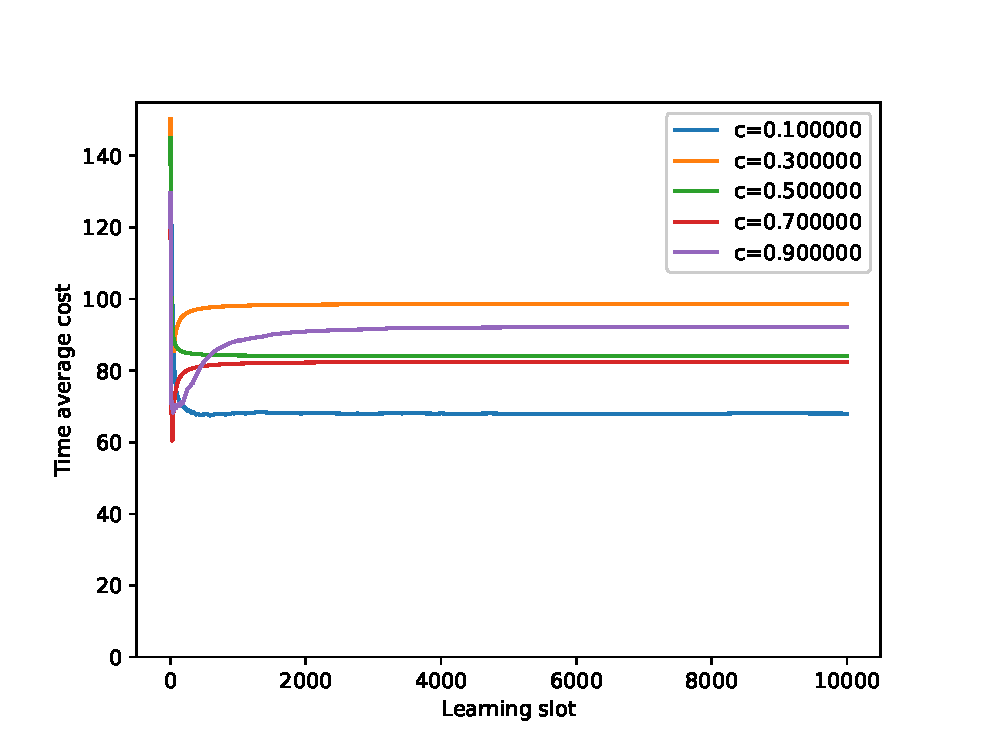
\includegraphics[width=0.9\linewidth]{figs/exploreratio1.eps}
%     \caption{effect of exploration ratio}
%     \label{fig:exploratio}
% \end{figure}

% \begin{figure*}[t]
%     \centering
%     \begin{subfigure}[b]{.45\textwidth}
%         \centering
%         \includegraphics[width=\linewidth]{figs/replotlearningnormalized.eps}
%         \caption{\myalgorithm approaching to the offline optimum}
%         \label{fig: mainlearning}
%     \end{subfigure}
%     \begin{subfigure}[b]{.45\textwidth}
%         \centering
%         \includegraphics[width=\linewidth]{figs/replotsingleregret.eps}
%         \caption{Total regret converges around 2000 learning slots}
%         \label{fig:regret}
%     \end{subfigure}
%     % \begin{subfigure}[b]{.32\textwidth}
%     %     \centering
%     %     \includegraphics[width=\linewidth]{figs/replotregret1.eps}
%     %     \caption{effect of exploration ratio}
%     %     \label{fig:exploratio}
%     % \end{subfigure}
%     \caption{Convergence performance}
%     \label{fig: Convergence performance}
% \end{figure*}





% \begin{figure}
%     \centering
%     \includegraphics[width=0.9\linewidth]{figs/replotregret.eps}
%     \caption{Regret analysis}
%     \label{fig:regretanalysis}
% \end{figure}
\subsection{Scalability Analysis}
In this section we analyze how \myalgorithm\ is affected by the scale of the problem and compare its performance with the two aforementioned greedy online approaches.

\subsection{Running Time Analysis}
In this experiment, we gradually increased the problem size and computed the running time and cost. 

We increase the network size from 3x3 to 6x6 nodes and specify the number of services on SFC from 3 to 10, then run \myalgorithm\ for 1000 learning slots and calculate the running time. The results are shown in figure \ref{fig:runtimeanalysis}, as expected from the complexity of algorithm \ref{alg:cccpa}, the running time is dominated by the number of available edge servers. Considering that there are 1000 times in this simulation, the average per-time-slot running time is less than 0.3 seconds, which is acceptable for any practical usages.
\begin{figure}
	\centering
	\includegraphics[width=.9\textwidth]{figs/replotruntime_smallfont.eps}
	\vspace{\baselineskip}
	\caption{Run time analysis}
	\label{fig:runtimeanalysis}
\end{figure}





% To analyze how number of services and edge computing nodes influence the algorithm run time, we compute the run time of \myalgorithm with different service number and node number, as shown in figure \ref{fig: runtimeanalysis}, the run time is more influenced by the number of nodes than services, this is due to the time complexity ($O(sn^2)$)of the oracle algorithm.


\subsection{Comparison with the greedy approaches.}
In this experiment, we further compare the cost of \myalgorithm\ with two greedy approaches to show our advantages on performance in terms of problem complexity. As it may be apparent, the difficulty of solving SFC orchestration in our problem depends on the number of services on SFC and the size of the network. Thus, we change these two parameters and see how it affects our algorithm and the greedy algorithms. As shown in figure \ref{fig: scalability}, with the complexity of the problem increases,  the performance of \myalgorithm\ is much less influenced than both greedy algorithms, which shows that our proposed algorithm has better scalability compared to the other two algorithms.
\begin{figure*}[t]
	\centering
	% \begin{subfigure}[b]{.45\textwidth}
	%     \centering
	%     \includegraphics[width=\linewidth]{figs/replotruntime.eps}
	%     \caption{Run time analysis}
	%     \label{fig:runtimeanalysis}
	% \end{subfigure}
	\begin{subfigure}[b]{.45\textwidth}
		\centering
		\includegraphics[width=\linewidth]{../icfec21/figs/numservicebar.eps}
		\caption{Number of services on SFC}
		\label{fig:numservicebar}
	\end{subfigure}
	\begin{subfigure}[b]{.45\textwidth}
		\centering
		\includegraphics[width=\linewidth]{../icfec21/figs/numnodebar.eps}
		\caption{Size of the MEC network}
		\label{fig:numnodebar}
	\end{subfigure}
	\vspace{\baselineskip}
	\caption{ Performance analysis under different problem scales: a) Number of services on SFC; b) Size of the MEC network}
	\label{fig: scalability}
\end{figure*}





% \begin{figure}
%     \centering
%     \includegraphics[width=0.9\linewidth]{figs/switchingcost.eps}
%     \caption{Multiple algorithms under different weights of switching cost}
%     \label{fig:switchweightbar}
% \end{figure}



% \section{Virtual cluster model}
% Future work discussion
% To simplify the network topology and reduce the number of link arms, we apply $Unison$\cite{vswitch} to convert the grid network topology to a virtual switch cluster topology that is shown in figure 9. All computing nodes including cloud will be connected via a vSwitch.

% \subsubsection{Estimation of the vSwitch and links}


% \begin{figure}
%     \centering
%     \includegraphics[width=0.7\textwidth]{virtualswitch2.png}
%     \caption{Virtual switch cluster}
%     \label{fig:my_label}
% \end{figure}
% \section{Alternative Approaches}
% Besides MAB, we can also apply Reinforcement learning in our model.







